\chapter{Perturbative Approach in Strong Lensing}
\section{Basic Ideas}
Let us assume that the projected density of the lens $\Sigma$ is axially symmetric
and centered at the origin. Let us assume that the lens is dense enough to
reach critical density at a given radius  $\re$. Under such hypotheses, the image
of a point source placed at the origin will be a perfect ring. However, if the
source is not be perfectly at the center and/or the potential maybe not be
perfectly circular, the perfect ring is broken in  arcs.

To investigate this fact, we will use the lens equation $\vec{r}_s = \vec{r} -
\vec{\alpha}$, where $\vec{r}_s$ is the angular position of the point
source in the source plane (see fig. in Narayan and Bartlemann for
this), $\vec{r} = r \hat{r} $ is the angular position of the point
source in the image plane, and $\vec{\alpha}$ is the deflection angle,
which is equal to the radial gradient of the 2D projected potential
$\phi$, which in polar coordinates is

\beq
\nabla_r \phi = \dfrac{\prtl  \phi}{\prtl r} \hat{r} + \dfrac{1}{r} \dfrac{\prtl  \phi}{\prtl \theta} \hat{\theta}.
\eeq

(also, we use $ \hat{r}, \hat{\theta}$ in place of Alard's $\hat{u_r}, \hat{u_\theta}$).

Thus
\bea
\vec{r}_s & = & r \hat{r} - \left( \dfrac{\prtl  \phi}{\prtl r} \hat{r} - {1 \over r} \dfrac{\prtl  \phi }{ \prtl \theta} \hat{\theta} \right) \label{eq:rs} \\
& = & \left( r -  \dfrac{\prtl \phi}{\prtl r} \right) \hat{r} -  \dfrac{1}{r} \dfrac{\prtl \phi }{\prtl \theta} \hat{\theta}
\eea

Now let's go to the simplest case of an on-axis point source with
perfectly axially symmetric potential $\phi = \phi_0$.  In this case
$r_s = 0, {\prtl \phi_0 \over \prtl \theta} = 0$ since there is no
angular variation of the potential.

Thus, eq.(\ref{eq:rs}) reduces to

\beq
0 =  r -  {\prtl  \phi \over \prtl r}
\eeq

or

\beq
\label{eq:einsteinradius}
  r =  \left. {\prtl  \phi \over \prtl r} \right|_{\re} = \re
\eeq

Where the derivative of the potential is to be evaluated at the Einstein radius, $ \re$.

This indicates the point source is spread into a circle of radius $ \re $ in the image plane.

We now take the first step of perturbing the situation:

\bea
\label{eq:rspert}
r_s & = & \eps y \\
\phi & = & \phi_0 + \eps \psi
\eea

which imply we have moved the source off-axis, and added a non-axially
symmetric potential, both to the exact same order $\eps$ by
assumption.  Note that the perturbed distance $y$ is in the source plane.

Note that this changes the notation of the first eq in Alard eq.3
(which is fairly nonsensical, of course).

Eq.(\ref{eq:rspert}) leads to a modification of eq.(\ref{eq:einsteinradius}) into

\beq
\label{eq:rpert}
r = \re + \eps x
\eeq

which changes the notation in Alard eq.4 (which is somewhat weird notation,
since his $dr$ is not necessarily a small distance), and we do not follow
his convention of setting $\re \equiv 1$.

Note that now the perturbed distance $x$ is in the image plane.

To recap: $r_s, y$ are in the source plane, while $r, x$ are in the image plane.

Now we do a Taylor series expansion of the potential:

\beq
\phi = \phi_0 + \eps \psi = \sum_{n=0}^\infty {1 \over n!} \left. {d^n \phi_0 \over dr^n }\right|_{\re} (r-\re)^n + \eps {1 \over n!} \left. {d^n \psi(\theta) \over dr^n }\right|_{\re} (r-\re)^n
\eeq

or

\beq
\label{eq:tse}
\phi  = \sum_{n=0}^\infty \left[ {1 \over n!} \left. {d^n \phi_0 \over dr^n }\right|_{\re} + \eps {1 \over n!} \left. {d^n \psi(\theta) \over dr^n }\right|_{\re} \right] (r-\re)^n
\eeq

And now define

\beq
C_n \equiv {1 \over n!} \left. {d^n \phi_0 \over dr^n }\right|_{\re}
\eeq

\beq
f_n(\theta) \equiv  {1 \over n!} \left. {d^n \psi(\theta) \over dr^n }\right|_{\re}
\eeq

So that we can write  eq.(\ref{eq:tse}) as

\beq
\label{eq:tse2}
\phi  = \sum_{n=0}^\infty \left[ C_n + \eps f_n  \right] (r-\re)^n
\eeq

where $f_n = f_n(\theta)$.

Now let's go back and substitute \eqref{eq:rspert}) and \eqref{eq:rpert}) into \eqref{eq:rs}) to find
\beq
\eps y = \left( \re + \eps x -  {\prtl  \phi \over \prtl r} \right) \hat{r} - {1 \over \re + \eps x}  {\prtl  \phi \over \prtl \theta} \hat{\theta}
\eeq

Now substitute \eqref{eq:tse2}) into this to find

\bea
\eps y = \left( \re + \eps x -  {\prtl \over \prtl r} \left( \sum_{n=0}^\infty \left[ C_n + \eps f_n  \right] (r-\re)^n  \right) \right) \hat{r} - \\
{1 \over \re + \eps x}  {\prtl  \over \prtl \theta} \left( \sum_{n=0}^\infty \left[ C_n + \eps f_n  \right] (r-\re)^n  \right)  \hat{\theta} \nonumber
\eea

Remembering that $C_n, f_n$ are independent of $r$, and using $r-\re = \eps x$ :

\bea
\label{eq:tse3}
\eps y = \left( \re + \eps x -   \sum_{n=0}^\infty \left[ C_n + \eps f_n  \right] n (\eps x)^{n-1}  \right) \hat{r} - \\
{1 \over \re + \eps x}  {\prtl  \over \prtl \theta} \left( \sum_{n=0}^\infty \left[ C_n + \eps f_n  \right] (\eps x)^n  \right)  \hat{\theta} \nonumber
\eea

Let us expand \eqref{eq:tse3}) in orders, first the zero'th order piece in $\eps$:


\beq
0 =  \left(\re - C_1 \right) \hat{r} \rightarrow \re = C_1 = \left. \prtl \phi \over \prtl \theta \right|_{\re}
\eeq


Next the first order piece in $\eps$:

\beq
\eps y = \left( \eps x - (2 C_2 \eps x + \eps f_1 ) \right) \hat{r} - {1 \over \re} \eps {\prtl f_0 \over \prtl \theta } \hat{\theta}
\eeq

where the coefficient of $C_2$ was expanded to order with $n=2$, that of the $f_1$ term with $n=1$, and that of the $\prtl f_1 \over \prtl \theta$ term with $n=0$.  Bit involved, but this is how to get each term proportional to $\eps$.

Now divide through by $\eps$ and collect terms:

\beq
 y = \left[ (1-2 C_2) x -  f_1 \right] \hat{r} - {1 \over \re} {\prtl f_0 \over \prtl \te} \hat{\theta}
\eeq

or, defining $\kt = 1-2 C_2$

\beq
\label{eq:rsexpanded}
 y = \left[ \kt x - f_1 \right] \hat{r} - {1 \over \re} {\prtl f_0 \over \prtl \te}  \hat{\theta}
\eeq

which is Alard eq.8 (remember he set $\re \equiv 1$).


\section{Conditions for the Validity of the Approximation}
%%%%%%%%%%%%%%%%%%%%%%%%%%%%%%% Habib

At first order in $\eps$ we may define

\begin{equation}
 q \equiv \frac{r}{\re}[1-\eps\,g(\te)].
\end{equation}

As the functional $\phi_0(q)$ represents the general expression
for the perturbed potential, with $q$ defined above, we may expand $\phi_0(q)$

\begin{displaymath}
 \phi_0(q)=\phi_0\left(\rre-\eps\rre\,g(\te)\right)
\end{displaymath}

\noindent in a Taylor Series around $\eps=0$, in the following way

\def\dpdq{ \left. \left( \frac{d\phi_0}{dq}\right) \right|_{\eps=0} }
\def\dpde{ \left. \left( \frac{d\phi_0}{d\eps}\right) \right|_{\eps=0} }

\begin{eqnarray}
 \phi_0(q) &\approx& \phi_0\prre+\eps \dpde \\
	  & = & \phi\prre+\eps \dpdq  \left(\frac{\prtl q}{\prtl \eps}\right)\\
	  &\approx& \phi\prre-\rre\phi_0^\prime\prre g(\te)\eps \label{key1}
\end{eqnarray}

Where we have defined $\phi_0^\prime\prre \equiv  \dpdq$.  Note, that we have $\phi_0(q)=\phi_0\prre$ when $\eps=0$ and similarly with its derivatives. Therefore,
taking the partial derivatives of Eq.~(\ref{key1}), it is straightforward to verify

\begin{eqnarray}
 \re\frac{\prtl \phi}{\prtl r}&=& \phi_0^\prime\prre -%
  \eps\left[g(\te)\phi_0^\prime\prre+\rre g(\te)\phi_0^{\prime \prime}\prre\right]\\
\frac{\re}{r}\frac{\prtl \phi}{\prtl \te}&=&-\phi_0^\prime\prre \frac{dg(\te)}{d\te}\eps
\end{eqnarray}

(Alard eq.19).

\section{Critic and Caustic Lines in the Perturbative Approach}

We will now obtain the equations of the critical curves in the lens
plane (corresponding to the caustic curves in the source plane).

First write \eqref{eq:rsexpanded} in Cartesian coordinates (expanding
the unit polar vectors, \eqref{eq:unitvs} ), changing notation
slightly, and taking $\vec{y}=(y_1,y_2)$ in the source plane and
$\vec{r}=(r,\te)$ in the lens plane:
%Note that as we have not considered the position of the source,
%we have $\bar{f}_i=f_i$ and therefore
\begin{eqnarray}
y_{1} &=& [\kt x - f_1]\cos{\te}+\frac{1}{\re}\frac{d f_0}{d\te}\sin{\te} \label{y_1}\\
y_{2} &=& [\kt x - f_1]\sin{\te}-\frac{1}{\re}\frac{d f_0}{d\te}\sin{\te} \label{y_2},
\end{eqnarray}

The Jacobian of the transformation from polar to Cartesian coordinates is given by

\begin{equation}
J=\frac{\prtl y_1}{\prtl r}\frac{\prtl y_2}{\prtl \te}-\frac{\prtl y_1}{\prtl \te}\frac{\prtl y_2}{\prtl r}.
\label{jacob}
\end{equation}

The critical lines are defined by the condition $J=0$. Now, we may easily verify that
\begin{eqnarray}
\frac{\prtl y_1}{\prtl r}&=& \frac{\kt}{\epsilon} \cos{\te}\label{dy1dx}   \\
\frac{\prtl y_2}{\prtl r}&=& \frac{\kt}{\epsilon} \sin{\te}\\
\frac{\prtl y_1}{\prtl \te}&=& \scriptf(\te)\sin{\te}+\scriptg(\te)\cos{\te}\\
\frac{\prtl y_2}{\prtl \te}&=& -\scriptf(\te)\cos{\te}+\scriptg(\te)\sin{\te}\label{dy2dte}
\end{eqnarray}

using \eqref{eq:rsexpanded}, ${\prtl \over \prtl r} ={ 1 \over \epsilon}
{\prtl \over \prtl x}$ ( from \eqref{eq:rpert} ) and defining the functions
$\scriptf$ and $\scriptg$ as

\begin{equation}
\scriptf(\te)=\frac{1}{\re}\frac{d^2f_0}{d\te^2}-(\kt x -f_1) \quad \textrm{and} \quad %
\scriptg(\te)=\frac{1}{\re}\frac{df_0}{d\te}-\frac{df_1}{d\te}
\end{equation}

Substituting eqs.~(\ref{dy1dx}-\ref{dy2dte}) into eq.~(\ref{jacob}), it is straightforward to verify that $J=-{\kt \over \eps} \scriptf(\te)$ and therefore on the critical curves where $J = 0$

\begin{equation}
x=\frac{1}{\kt}\left[f_1+\frac{1}{\re}\frac{d^2f_0}{d\te^2}\right] \label{xte}.
\end{equation}

This is Alard eq. 30. From this last equation, the tangential critical curve can be expressed
in parametric form as
\beq
\vec{r}_{\mathrm{crit}}= \left[(\re +x)\cos{\te},(\re+x)\sin{\te}\right],\quad 0 \leq \te < 2\pi.
\eeq

Now, substituting this last equation into eqs.~(\ref{y_1}) and (\ref{y_2}) we obtain, the parametric equation for
the tangential caustic, i.e.,

\begin{eqnarray}
y_{1_\mathrm{caust}} &=& \frac{1}{\re}\frac{d^2f_0}{d\te^2}\cos{\te}+\frac{1}{\re}\frac{df_0}{d\te}\sin{\te}\\
y_{2_\mathrm{caust}} &=& \frac{1}{\re}\frac{d^2f_0}{d\te^2}\sin{\te}-\frac{1}{\re}\frac{df_0}{d\te}\cos{\te}
\end{eqnarray}

These last equations are Alard eqs. (31).

%%%%%%%%%%%%%%%%%%%%%%%%%%%%%%%%%  From before

Getting Alard eq.33 from 31 is straight, and then I (MSSG) got most of the way to
A.eq.34 from 33 and 32, with some small hiccups..

\section{Reconstruction of Images}

One advantages of this perturbative approach is allow us construct the lensed images
from sources located near to the tangential caustic.  In this section we
study the mapping of a circular and elliptical contour using this formalism.

\begin{wrapfigure}{r}{0.4\textwidth}
  \begin{center}
%  \centering{\epsfig{Fig_subsstructure.eps,width=0.45\textwidth}}
   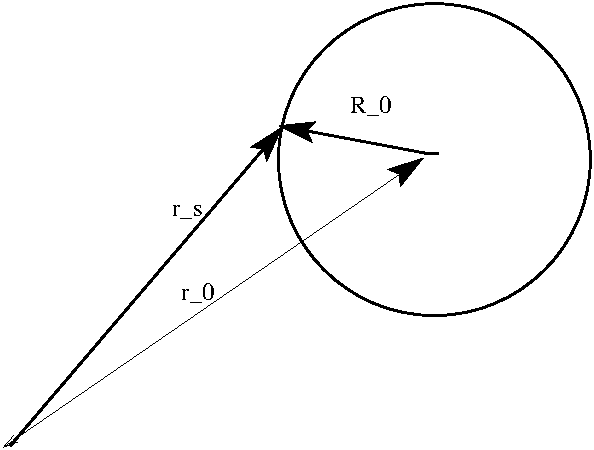
\includegraphics[width=0.35\textwidth]{graphics/sourceplane.pdf}
  \end{center}
    \caption{\label{circular_source}Circular source in the source plane.}
\end{wrapfigure}

Notation: $ \vec{r}_{0}$ points from the origin (i.e center of the
source plane, looking directly on-axis from us through the lens to the
source) to the center of the actual source object (like a small
circular galaxy), $ \vec{R}_{0}$ is the vectorial radius of this
source from its center, and $ \vec{r}_{s}$ is the vector from the
origin to some point on the edge of the circular source. As a first
stab, see \ref{circular_source} for this configuration.

So:

\beq
\vec{r}_s =  \vec{r}_{0} + \vec{R}_{0} , \quad \rightarrow \vec{R}_{0} = \vec{r}_s - \vec{r}_{0}.
\eeq


Replacing $r_s$ by \eqref{eq:rsexpanded}), we obtain:

\beq
\label{eq:Rzero}
\vec{R_{0}} = \left[ \kappa_2 x - f_{1}(\theta) \right]\hat{r} - \frac{1}{\re} \frac{\partial f_0(\theta)}{\partial \theta} \hat{\theta} - \vec{r_{0}}. \;\;\;
\eeq


Note that $\vec{r}_{0} = (x_0,y_0)$ lies in the source plane, but we
can write it in terms of the polar unit vectors

\bea
\label{eq:unitvs}
\hat{r}=(\cos\te, \sin \te) \\
\hat{\theta}=(-\sin \te, \cos \te)
\eea

 as following

\beq
\vecrz = (\vecrz \cdot \hatth) \hatth + (\vecrz \cdot \hatr) \hatr
\eeq

or

\beq
\label{eq:rzero}
\vec{r}_{0} = \left[ x_0 \,  \cos \te + y_0 \,  \sin \te \right] \hat{r} + \left[ -x_0 \,  \sin \te + y_0 \,  \cos \te \right] \hat{\theta}.  \;\;\;
\eeq

So that \eqref{eq:Rzero}) becomes

\beq
\vec{R_{0}} = \left[ \kappa_2 x - f_{1}(\theta) \right]\hat{r} - \frac{1}{\re} \frac{\partial f_0(\theta)}{\partial \theta} \hat{\theta} -  \left[ x_0 \,  \cos \te + y_0 \,  \sin \te \right] \hat{r} + \left[ -x_0 \,  \sin \te + y_0 \,  \cos \te \right] \hat{\theta} \;\;\;
\eeq


Defining

\beq
\overline{f}_i(\theta) = f_i(\theta) + (x_0 \cos \te + y_0 \sin \te)\re^{1-i}, \;\; i=0,1
\eeq

this becomes

\beq
\vec{R}_{0} = \left[ \kappa_2 x - \overline{f}_{1}(\theta) \right]\hat{r} - \frac{1}{\re} \frac{\partial \overline{f}_0(\theta)}{\partial \theta} \hat{\theta}. \;\;\; \label{Eq_Alard11}
\eeq

(Alard eq.11).

Now, taking the square of this we obtain

\beq
R_{0}^2 = \left[ \kappa_2 x - \overline{f}_{1}(\theta) \right]^2 + \left[\frac{1}{\re} \frac{\partial \overline{f}_0(\theta)}{\partial \theta}\right]^2. \;\;\;
\eeq

Solving this for $x(\te)$, the radius of the arc in the image plane as
a function of theta, the following two solutions are obtained:

\beq
\label{eq:xsoln}
x = \frac{1}{\kappa_2}\left[ \overline{f}_{1}(\theta) \pm \sqrt{R_0^2 - \left( \frac{1}{\re}\frac{\partial \overline{f}_0(\theta)}{\partial \theta} \right)^2} \right]. \;\;\;
\eeq

corresponding to the inner and outer edges of the arc.

Thus, given the source radius $R_{0}$ and position $(x_0,y_0)$ we can
draw the arcs using \eqref{eq:xsoln}). The parametric equation for the
arcs (or images) are defined as

\beq
\vec{r}= \left[(\re +x)\cos{\te},(\re+x)\sin{\te}\right], \quad 0 \leq \te < 2\pi.
\eeq


\subsection{Elliptical Source Contours}
%%%%%%%%%%%%%%%%%%% Gabriel
{\bf If someone have doubts about this procedure, let me know \ldots}

We now extend the discussion of previous section to elliptical contours.

First we can consider the vectorial equation of an elliptical contour aligned to
the main axis (note that this is a very limited set of ellipses),

\beq
\label{eq:ellipse}
\vec{R}_0=\left(\sqrt{1-\eta_s}y_{1s},\sqrt{1+\eta_s}y_{2s}\right)
\eeq
where $\eta_s$ is the ellipticity of the source, $R_0$ is the characteristic size of the source
and $y_{is} = (\vec{r}_s-\vec{r}_0)\cdot\hat{i}$ ($\hat{i}=(1,2)=(\hat{\imath},\hat{\jmath})$).

From Eq.~(\ref{Eq_Alard11}) and writing the polar unitary vectors in cartesian components we get to

\bea
y_{1s}&=&(\kt x -\bar{f}_1)\cos{\te}+\frac{1}{\re}\dfrac{\prtl \bar{f}_0}{\prtl \te}\sin{\te} \label{y_1s}\\
y_{2s}&=&(\kt x -\bar{f}_1)\sin{\te}-\frac{1}{\re}\dfrac{\prtl \bar{f}_0}{\prtl \te}\cos{\te} \label{y_2s}.
\eea

Defining

\bea
\bar{y}_{1s}&=&\kt x -\bar{f}_1\label{bar_y1}\\
\bar{y}_{2s}&=&\frac{1}{\re}\dfrac{\prtl \bar{f}_0}{\prtl \te},\label{bar_y2}
\eea
we can express $\vec{R}_0$ as

\beq
\vec{R}_0=\left[\sqrt{1-\eta_s}(\bar{y}_{1s}\cos{\te}+\bar{y}_{2s}\sin{\te}) \right]\hat{\imath}+\left[\sqrt{1+\eta_s}(\bar{y}_{1s}\sin{\te}-\bar{y}_{2s}\cos{\te}) \right]\hat{\jmath}
\eeq

Taking square of the equation above and solving for $\bar{y}_{1s}$, is straightforward to verify

\beq
\bar{y}_{1s}=\dfrac{\eta_s\cos{(2\te)}}{S}\bar{y}_{2s}\pm \frac{1}{S}\sqrt{S R_0^2-(1-\eta_s)\bar{y}^2_{2s}}
\eeq

where $S=1-\eta_s\cos{(2\te)}$. Replacing the Eq.~(\ref{bar_y1}) and Eq.~(\ref{bar_y2}) in the equation above, we get to

\beq
x = \frac{1}{\kappa_2} \left\{\bar{f}_{1}(\theta) + \frac{\eta_s\sin(2\theta)}{S}\left(\frac{1}{\re}\dfrac{\partial \bar{f}_0(\theta)}{\partial \theta}\right) \pm \frac{1}{S}\sqrt{SR_{0}^2 - (1-\eta_s^2)\left[ \frac{1}{\re}\frac{\partial \bar{f}_0(\theta)}{\partial \theta}\right]^2}  \right\}.
\label{elliptical_contour}
\eeq

The parametric equation for the images of elliptical sources is

\beq
\vec{r}= \left[(\re +x)\cos{\te},(\re+x)\sin{\te}\right], \quad 0 \leq \te < 2\pi.
\eeq

{\bf New}

In the general case, when the source is not aligned to the main axis ( the source is oriented in an angle
$\te_0$), the vectorial equation of an elliptical contour is

\beq
\label{eq:ellipsetheta}
\vec{R}_0=\left(\sqrt{1-\eta_s}y^\prime_{1s},\sqrt{1+\eta_s}y^\prime_{2s}\right)
\eeq
where, $y^\prime_{is}\, (i=1,2)$ are obtained rotating the coordinate system of the source in an angle $\te_0$,
i.e
\begin{equation}
\left(\begin{array}{c}y^\prime_{1s} \\ y^\prime_{2s} \end{array}\right)=\left[\begin{array}{c c}%
\cos{\te_0} & \sin{\te_0}\\ -\sin{\te_0} & \cos{\te_0} \end{array} \right]\left( \begin{array}{c} y_{1s}\\ y_{2s}\end{array}\right)
\end{equation}

Using the Eqs.~(\ref{y_1s}-\ref{bar_y2}) is easily to verify
\bea
y^\prime_{1s}&=&\bar{y}_1\cos{\tilde{\te}}+\bar{y}_2\sin{\tilde{\te}}\\
y^\prime_{2s}&=&\bar{y}_1\sin{\tilde{\te}}-\bar{y}_2\cos{\tilde{\te}}\\
\tilde{\te}&\equiv&\te-\te_0
\eea

Now, following the procedure showed above, is straightforward get to the expression for the images coming from
lensed elliptical sources (with orientation $\te_0$), and is given by the Eq.(\ref{elliptical_contour}) with $\te$ replaced by $\tilde{\te}$
adequately, i.e

\bea
x &=& \frac{1}{\kappa_2} \left\{\bar{f}_{1}(\theta) + \frac{\eta_s\sin(2\tilde{\theta})}{S}\left(\frac{1}{\re}\dfrac{\partial \bar{f}_0(\theta)}{\partial \theta}\right) \pm \frac{1}{S}\sqrt{SR_{0}^2 - (1-\eta_s^2)\left[ \frac{1}{\re}\frac{\partial \bar{f}_0(\theta)}{\partial \theta}\right]^2}  \right\}.\label{elliptical_contour2}\\
S&\equiv& 1-\eta_s\cos{(2\tilde{\te})}
\eea
This is the Eq. (28) of Pierani et al. 2008 (remember again, they set $\re=1$ and $\eta_s=\sqrt{2\eta_0}$)

%\beq
%\label{eq:ellipse}
%(1-\eta_s)x_s^2 + (1+\eta_s)y_s^2 = R_{0}^2.\;\;\;
%\eeq

As we can see, the condition for the formation of images is given by
\begin{equation*}
S\,R^2_0>(1-\eta^2_s)\left[\frac{1}{\re}\dfrac{\prtl \bar{f}_0}{\prtl \te}\right]^2
\end{equation*}

And therefore, the number of images is given by the quantity of times that the expression above is $0$ or negative.

\section{Measurements of the arc properties}

Here, I or we will put the analytical expression for the Length and Width or arcs.

\section{Inverse Modelling}

To get Alard eq.29, take Alard eq. 12:


\beq
x = \frac{1}{\kappa_2}\left[ \overline{f}_{1}(\theta) \pm \sqrt{R_0^2 - \left( \frac{1}{\re}\frac{\partial \overline{f}_0(\theta)}{\partial \theta} \right)^2} \right]. \;\;\; 
\eeq

And separate the two solutions for the inner and outer edge of the arc:



\bea
x_i = \frac{1}{\kappa_2}\left[ \overline{f}_{1}(\theta) - \sqrt{R_0^2 -%
\left( \frac{1}{\re}\frac{\partial \overline{f}_0(\theta)}{\partial \theta} \right)^2} \right]. \;\;\;  \\
x_o = \frac{1}{\kappa_2}\left[ \overline{f}_{1}(\theta) + \sqrt{R_0^2 - %
\left( \frac{1}{\re}\frac{\partial \overline{f}_0(\theta)}{\partial \theta} \right)^2} \right]. \;\;\;  
\eea


Take 

\beq
x_o + x_i = {2 \over \kappa_2} \fbar 
\eeq

And solve for $\fbar$:


\beq
\fbar = {\kappa_2 \over 2} (x_o+x_i)
\eeq

which is exactly Alard eq. 29a, without his additional constant (whose provenance I don't get at the moment).

Now take 

\beq
x_o - x_i = {1 \over \kappa_2} \left(2 \sqrt{R_0^2 - {\left( {1 \over \re} \dfdt \right)}^2 }\right)
\eeq

And solve for $\dfdt$ (few straight steps of algebra here):

\beq
\dfdt = \re \sqrt{R_0^2 - {\kappa_2^2 \over 4} (x_o-x_i)^2 }
\eeq

which is our form of Alard eq. 29b.

\section{Errors on arcs}
%%%%%%%%%%%%%%%%%%%%%%%%%%%%%%% Marcos

Recall that $\phi=\phi_0+\eps\psi$ and expand only $\psi$:

\beq
\phi=\phi_0+\eps\sum_{n=0}^{\infty}f_n(\theta)(r-\re)^n
\eeq

Differentiating we obtain

\bea
\frac{\partial \phi}{\partial r }&=&\phi_0^\prime+\eps\sum_{n=1}^{\infty}f_n(\theta)n(r-\re)^{n-1} \\
\frac{\partial \phi}{\partial \theta}&=&\eps\sum_{n=0}^{\infty} \frac{\partial f_n}{\partial \theta}(r-\re)^n
\eea

Evaluating at the Einstein radius $r=r_{\mathrm{E}}$, we have

\bea
\frac{\partial \phi}{\partial r }&=&\phi_0^\prime+f_1(\theta) \\
\frac{\partial \phi}{\partial \theta}&=&\eps \frac{\partial f_0}{\partial \theta}
\eea

On the other hand, evaluating Eqs. 19 in Alard at $r=\re$, and using Eq. 16 in Alard $\phi_0^\prime=1+2C_2(r-r_{\mathrm{E}}+...$ 

\bea
\frac{\prtl \phi}{\prtl r}&=& \phi_0^\prime -%
  \eps g(\te)\left[\phi_0^\prime+ \phi_0^{\prime \prime}\right]=\phi_0^\prime-\eps g(\te)(1+C_2)\\
\frac{\prtl \phi}{\prtl \te}&=&-\eps\phi_0^\prime \frac{dg(\te)}{d\te}
\eea

Comparing these equations, we have a relation between the $f_n(\te)$ and $g(\te)$ functions:

\bea
f_1&=&-(1+2C_2)g \\
\frac{df_0}{d\theta}&=&-\frac{dg}{d\theta}
\eea

Eq. (30) in Alard (to be derived later) is

\beq
dr=\frac{1}{\kappa_2}\left[ f_1+\frac{d^2f_0}{d\theta^2} \right]
\eeq

and in this case we have

\beq
dr=\frac{1}{\kappa_2}\left[ -(1+2C_2)g+\frac{d^2g}{d\theta^2} \right]
\eeq

Not sure what the effective parameter $dr_c$  in Eq 22 is and how to get it.
Assuming it's correct, i.e.
\beq
dr_c\sim -\frac{d^2g}{d\te^2}-2g
\eeq
we have that for e.g. the NFW profile with ellipticity (as in Eq. 28 of Alard)

\bea
\phi_0(q)&=&\frac{1}{2}\log^2\left(\frac{q}{2}\right)-2\arctan^2\left(\sqrt{\frac{1-q}{1+q}}\right) \\
q&=&u_0r\sqrt{1-\eta\cos(\theta)}\approx u_0 r \left[1-\frac{\eta}{2}\cos(2\theta)\right]
\eea

So in this case we have (notice $\eta/2$ plays the role of $\eps$ here, so only expect expansion to work 
for small ellipticities)

\bea
g(\te)&=&\frac{\eta}{2}\cos(2\theta) \\
\frac{d^2g(\te)}{d\te^2}&=&-2\eta\cos(\theta)=-4g
\eea

so that $dr_c=\eta\cos(\theta)$. Not sure if this is true for any elliptical potential or if it's specific to NFW.
In any case the deviation is maximum for $\te=0,\pi$

If the Taylor expansion converges, truncating it at some order has a maximum error given by the next order 
term. In this case the maximum error due to the non-linearity of the gradient of the potential is 

\beq
D=3C_3\max[dr_c^2]=3C_3\eta^2
\eeq

Notice it increases with the ellipticity squared. For a general potential of the form

\beq
\phi=\frac{1}{\alpha}r^{\alpha[1+\beta(r-1)]}
\eeq

we have

\beq
C_3=\frac{d^3\phi}{dr^3}|_{r=1}=-\frac{(\alpha-1)}{6}+\frac{\beta}{2}
\eeq

and $D^2$ follows. 




